\subsection{Specific Aim 3: Self-assembly of Janus particles in ionic solutions}
\label{subsec:specific_aim_3}

\subsubsection{Dynamics of a pair of Janus particles in ionic solutions\label{subsubsec:JP_electrolyte}}
In experiments, Janus particles are often immersed in a solution of ions \cite{Chen2011_Science} or surfactants \cite{Goodwin2009}.
In electrolytic solutions the interaction between salt and Janus particle gives 
rise to a slip velocity (on the particle surface) that depends on the ion distribution and the zeta potential \cite{BayatiNajafi2016_JCP} 
(the potential difference between the Janus particle surface and the surrounding conducting fluid).
The short-range interactions between Janus particles depend on the salt concentration:
At very low salt concentrations, Janus particles repel one another electrostatically, whereas at high salt concentration, van der Waals
forces cause Janus particles to aggregate irreversibly \cite{Goodwin2009}. At intermediate concentrations of monovalent salt, Janus particles are found to assemble in the form of a small number of elemental units of building blocks \cite{Chen2011_Science}. 
%
\begin{wrapfigure}[7]{r}{0.45\textwidth}
  \vspace{-5pt}
\centerline{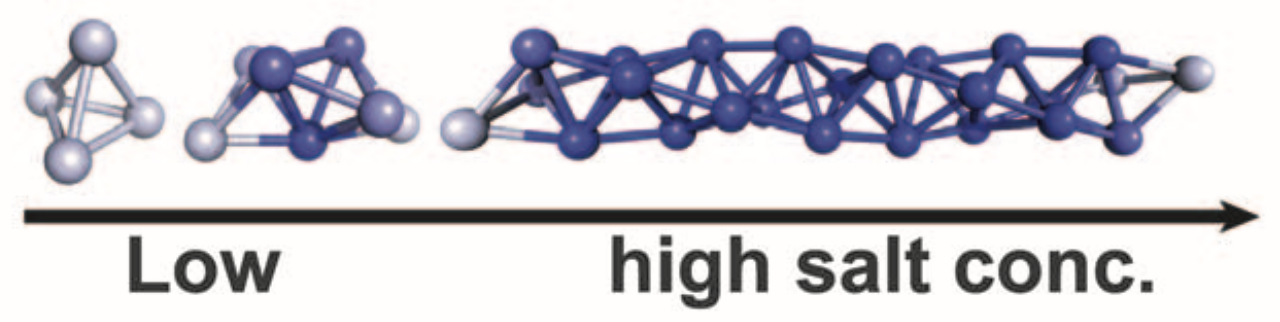
\includegraphics[width=0.44\textwidth]{Figures/fig2A_Chen2011_Science}}
  \vspace{-5pt}
\caption{\label{fig:helices_of_JPs} \footnotesize Formation of helices of Janus particles as salt concentration increases from 3.8 mM NaCl  (left) to 5 mM NaCl (right)\cite{Chen2011_Science}.}
\end{wrapfigure}
%
Figure~\ref{fig:helices_of_JPs} shows that Janus particles can assemble into a helix at high concentration of monovalent salt (NaCl) when the volume fraction of Janus particles is low to moderate. At high volume fraction, helices of Janus particles form wormlike structures whose lifetime allow fusion of helices \cite{Chen2011_Science}. 

We propose to investigate the effects of ion transport and distribution on the self-assembly of Janus particles within the HAP framework as follows.
First the Stokes equations are modified to incorporate the transport of ions as
\begin{equation}
\label{eq:EKstokes}
\begin{aligned}
  &-\Delta \mathbf{u} + \nabla p = \Delta\psi\cdot\nabla\psi, \qquad
  \nabla \cdot \mathbf{u} = 0,  \quad \mathbf{x} \in \Omega,\\
  &\delta^2\Delta\psi = -\frac{1}{2}\left(n_+-n_-\right),\qquad
  \frac{\partial n_{\pm}}{\partial t} + \nabla\cdot{\bf j}_{\pm} = 0,\qquad {\bf j}_{\pm} = -\nabla n_{\pm} \mp n_{\pm} \nabla\psi + \mbox{Pe} n_{\pm}\mathbf{u},
\end{aligned}
\end{equation}
where $\delta$ is the ratio of Debye screening length (inversely proportional to the square root of
ion concentration) to the particle size, 
$\mbox{Pe}$ is the Peclet number, a ratio between the convection and  thermal diffusion time scales.
$n_{+}$ ($n_{-}$) is the concentration of cation (anion).  In the limit of small $\delta$, PI Young and collaborator Y. Mori (U Penn) used asymptotic analyses to show that the jump in electric potential $\psi$ across the interface (zeta potential on the Janus particle surface) 
may give rise to different physical consequences such as electrophoresis \cite{Mori2018_JFM}.
%
An important question to address is: {\it How would such electrophoresis be affected by the HAP between two Janus particles?} 
As the first part of specific aim 3, we will address this important question. Results from this effort will help elucidate the effects of salt concentration on the assembly of Janus particles (\S~\ref{subsubsec:em_effects}).

We couple the electrokinetics in~\eqref{eq:EKstokes} with the mobility  problem of Janus particles in a viscous solvent through the velocity field, ion distribution, and the hydrophobic potential.  
First the screen length $\rho$ in the HAP model is now a function of the  cation concentrations: $\rho = \rho(n_+) =
\rho_0/\sqrt{1+c n_+}$ with a dimensionless parameter $c$. 
%
Secondly the value of the HAP may depend on the distribution of ions and electric potential right next to the particle surface \cite{Mori2018_JFM}.
Within this framework, we will first investigate the interaction between two Janus particles under HAP in an electrolytic solution described by the above
equations. We will conduct analytical calculations to investigate the effects of ion transport on the hydrophobic attraction between two Janus particles using the reciprocal theorem as in \cite{BayatiNajafi2016_JCP} for two Janus particles with a small surface activity.



\subsubsection{Electromechanical effects on the dynamic assembly of Janus particles \label{subsubsec:em_effects}}
Results from the proposed work in \S~\ref{subsubsec:JP_electrolyte} will shed light on how the electrokinetics described in~\eqref{eq:EKstokes}
may be simplified to a dielectric-like model where the bulk charges are constant, and the fluid flow and particle mobility are determined by the surface charge and the zeta potential as shown in \cite{Mori2018_JFM}. Under such simplification, the modified~\eqref{eq:EKstokes} may be re-formulated into integral forms. PIs Ryham and Young will conduct the asymptotic analyses to derive the modified~\eqref{eq:EKstokes}, and work with PI Quaife to design a numerical algorithm to simulate the modified system using integral formulation. We will first investigate the effects of salt concentration on the assembly of Janus particles to form helices, as shown in figure~\ref{fig:helices_of_JPs}.

With these results, the PIs will be ready to make quantitative connections between the a Janus particle membrane and a lipid bilayer membrane in an electrolytic solution. In recent experiments~\cite{FaizEtAl2019_SoftMatt}, membrane bending
rigidity was determined as a function of lipid composition from 0 to 100
mol $\%$ of charged lipids using flicker spectroscopy of the shape
fluctuations of a giant unilamellar vesicle (GUV).
%the bending rigidity is determined as a
%function of lipid composition from 0 to 100 mol $\%$ of charged lipids
%in recent experiments~\cite{FaizEtAl2019_SoftMatt}---
Membrane bending rigidity increases with increasing lipid surface
charge, but decreases with increasing salt concentration in the bulk
solution due to the screening of the lipid surface charge. This
result agrees
with several theoretical models~\cite{Kralchevsky1996_JCIS,
May1996_JChemPhys, LoubetEtAl2013_PRE} that also assume the quadratic
form of the elastic energy density in the presence of surface charge and
bulk charge~\cite{DuplantierGoldstein1990_PRL, Winterhalter1992_JPC}. As
the electrostatic interaction is non-local in nature, we expect that the
controversy of the HK elastic energy form (see
\S\ref{subsec:specific_aim_1}) would worsen in the presence of
electrostatic interactions and electrokinetics. The PIs will extend the
approaches in \S\ref{subsec:specific_aim_1} to charged lipids to
calculate the bending moduli and compare against the experimental
results in~\cite{FaizEtAl2019_SoftMatt}. We propose to incorporate an
explicit surface charge on each particle boundary $P_i$ and compute the
electrostatic potential as a functional of particle configuration.
Adding the electrostatic force to the hydrophobic attraction force
between particles, we will assess the dependence of elastic moduli on
electric charges using the methods described in
\S\ref{subsec:specific_aim_1}. Results from these proposed calculations
will provide further comparisons and validations of the HAP model
against the continuum mechanics.

Once the effects of lipid charges on the moduli are verified, the PIs
propose to examine how to use an external electric field to control the
amphiphilic self-assembly in solvent. PI YNY has a track record of
working on electrohydrodynamics of an elastic, inextensible membrane
using both asymptotic analysis~\cite{Nganguia2013_PRE, Young2014_JFM,
Young2015_PoF} and numerical simulations~\cite{Nganguia2015_CiCP} and
will work with both PIs RR and BQ to extend the HAP model to study the
electromechanical effects on the assembly of amphiphile. Results from
this research will yield a quantitative understanding of how to utilize
an electric field to achieve optimal control of assembly of amphiphiles
in solvent.




